\documentclass[9pt]{beamer}

\usepackage[T1]{fontenc}
\usepackage{color}
\usepackage{graphicx}
\usepackage{natbib}
\usepackage{tikz}


\usetheme{Boadilla}

\usefonttheme{professionalfonts}

\title[Air Quality]{Air Quality - Agricultural Emissions}
\subtitle{}
\author{Max Callaghan}
\institute[MCC-Berlin]%{\includegraphics[height=1cm,width=2cm]{/home/max/Pictures/MCC_Logo_RZ_rgb.jpg}}

\newtheorem*{remark}{}

\bibliographystyle{apalike}

\begin{document}
	
\begin{frame}
	\titlepage
\end{frame}

\addtobeamertemplate{frametitle}{}{%
	\begin{tikzpicture}[remember picture,overlay]
	%\node[anchor=north east,yshift=2pt] at (current page.north east) {\includegraphics[height=0.8cm]{/home/max/Pictures/MCC_Logo_RZ_rgb.jpg}};
	\end{tikzpicture}}

\begin{frame}{Agricultural Emissions}
	
	Outdoor air pollution contributes to millions of global premature deaths annually, with  most health impacts air linked to fine particulate matter (PM\textsubscript{2.5}) \citep{Lelieveld2015}. 	Due to atmospheric reactions between alkaline ammonia (NH\textsubscript{3}) and acidic nitrogen oxides (NO\textsubscript{x}) and sulphur dioxide (SO\textsubscript{2}), that contribute to the formation of PM\textsubscript{2.5}, an optimal air pollution mitigation strategy should consider agricultural emissions (which primarily account for ammonia) as well as those from the transport and power sectors \citep{Wang2015, Lee2015}. Ammonia's contribution to premature mortality varies by region; in parts of Europe and North-Eastern America, reductions in Ammonia emissions may generate the largest reductions in mortality, although these results are sensitive to uncertainties about the relative toxicity of PM\textsubscript{2.5} particles by source \citep{Lee2015, Lelieveld2015}. Mitigation options for ammonia emissions are higher than other sectors, but behavioural changes towards reducing meat consumption would be highly effective, and would also generate health benefits for humans, a reduction in GHG emissions, a reduction in biodiversity loss, and the improvement of water quality \citep{Backes2016, Leip2015}.  

\end{frame}

\begin{frame}{Agricultural Emissions}

\begin{figure}
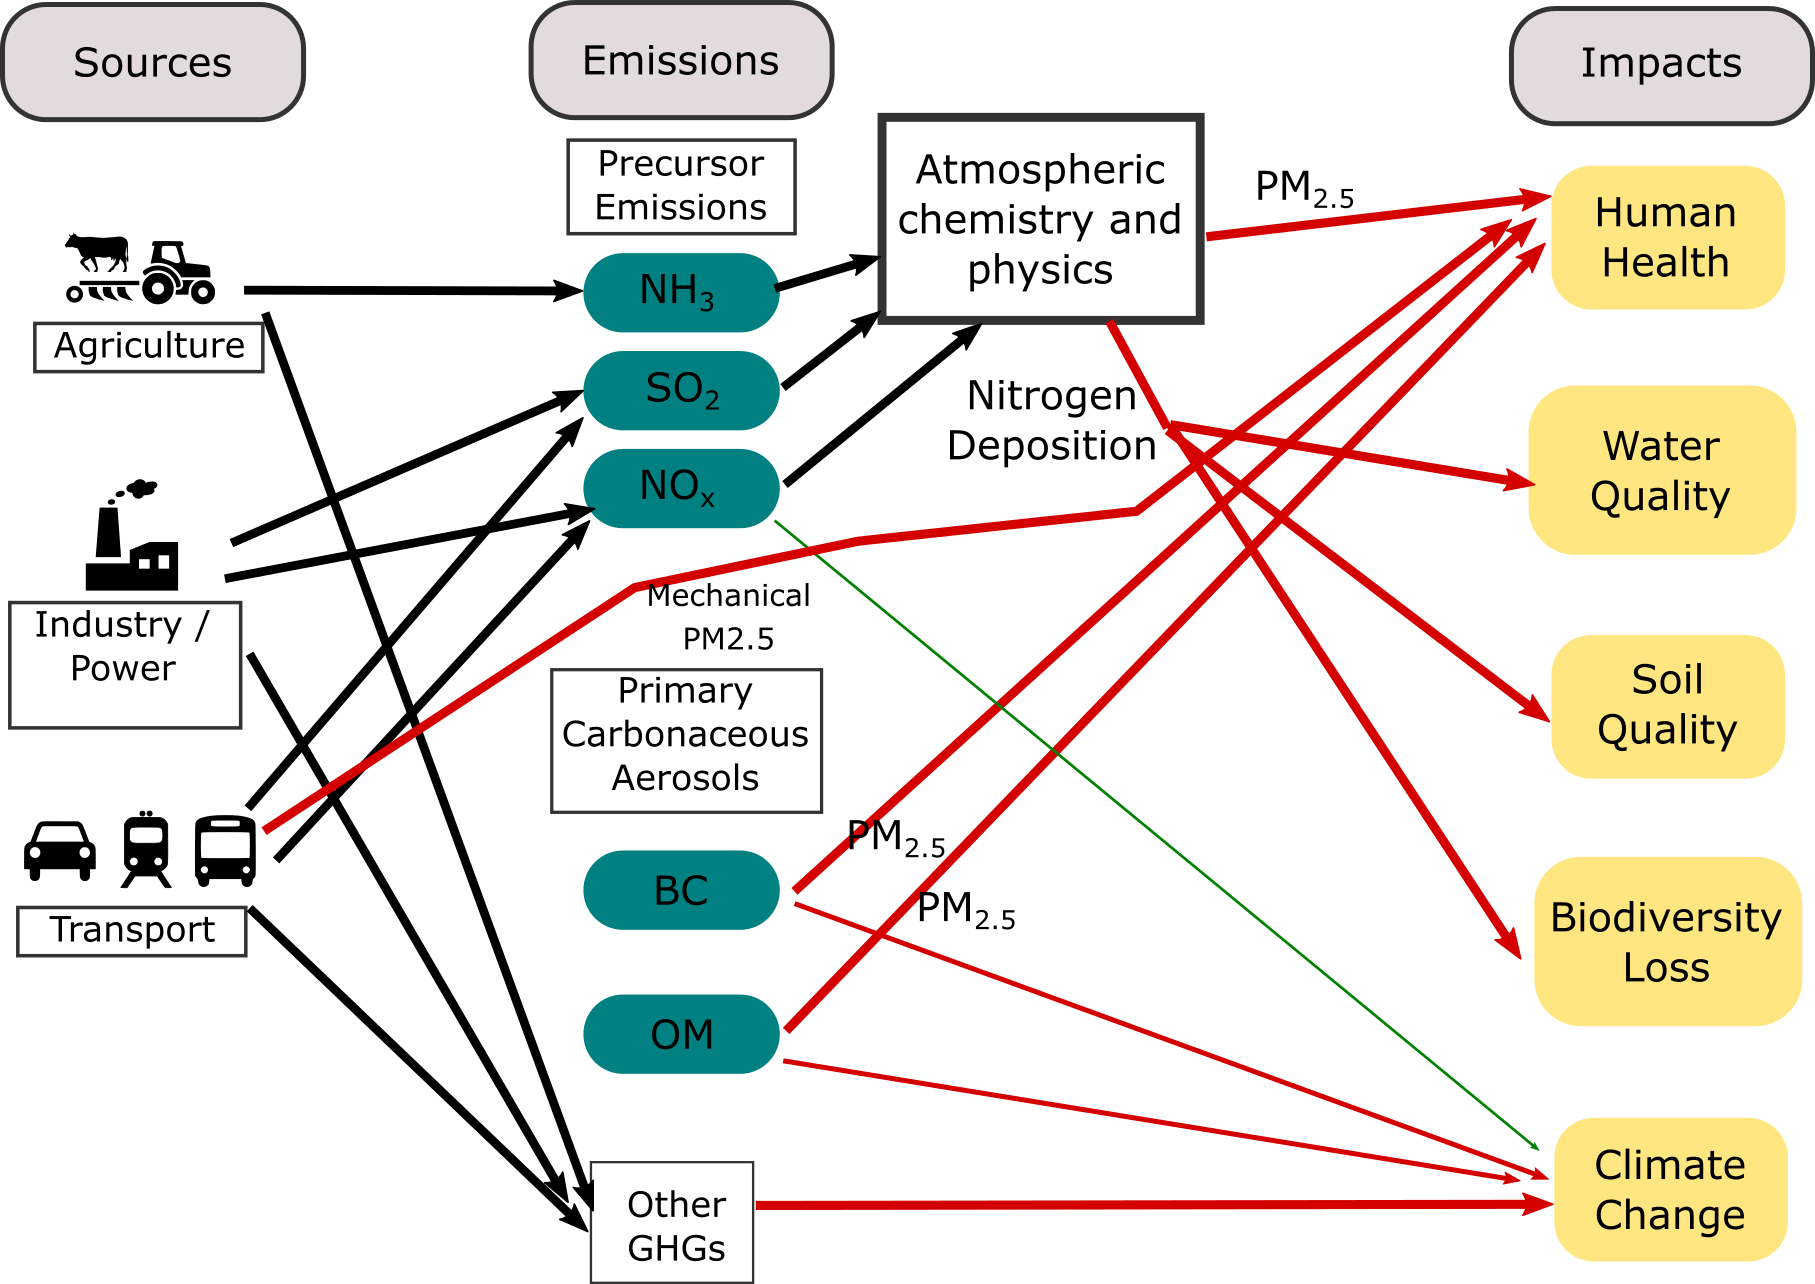
\includegraphics[height=7cm]{../ammonia.png}
\end{figure}
\end{frame}

\begin{frame}{Bibliography}
	\small
	\bibliography{/home/max/Documents/library/bibliography/airquality}
\end{frame}

\end{document}
